\documentclass[a4paper,12pt]{article}
\usepackage{amsmath}
\usepackage{amssymb}
\usepackage{graphicx}
\usepackage{geometry}
\usepackage{xcolor}
\usepackage{float}
\usepackage{hyperref}
\geometry{margin=1in}

\title{Control Systems Project Report}
\author{Syed Fahd Ali \\ Section C, DCSE \\ Enrollment Number: 21PWCSE1992}
\date{January 8, 2024}

\begin{document}

\maketitle

\section*{1. Problem }
Consider the following system with state-space representation for an inverted pendulum:
\begin{enumerate}
    \item Check the stability of the system using all known methods.
    \item Simulate the unstable system and show that its response is unstable.
    \item Compute the controllability and observability of the system. If the system is controllable, place the controller poles at $(-4,-3,-8,-5)$ and observer poles at locations faster than the controller poles.
    \item Simulate the stable system .Design a  PID controller also.
    \item Compute the steady state errors before and after designing controlles.
\end{enumerate}
\section*{2. Solution}

\subsection*{2.1 State-space Representation}
The state-space representation of the given system is:
\[
\dot{x} = Ax + Bu, \quad y = Cx + Du
\]
Where the matrices are:
\[
A = 
\begin{bmatrix}
0 & 1 & 0 & 0 \\ 
0 & -0.818 & 2.6727 & 0 \\ 
0 & 0 & 0 & 1 \\ 
0 & -0.4545 & 31.1818 & 0
\end{bmatrix}, \quad
B = 
\begin{bmatrix}
0 \\ 1.8182 \\ 0 \\ 4.5455
\end{bmatrix}
\]
\[
C = \begin{bmatrix} 1 & 0 & 0 & 0 \end{bmatrix}, \quad
D = 0
\]

\subsection*{2.2 Stability Analysis}
The eigenvalues of the system matrix \(A\) are:
\[
\lambda = \{0, 5.5670, -5.6067, -0.7783\}
\]
The poles of the transfer function are:
\[
\text{Poles} = \{0, 5.5670, -5.6067, -0.7783\}
\]
As one eigenvalue and one pole have positive real parts, the system is unstable in open-loop configuration.
The Step Response of the system shows that system is unstable in open-loop configuration.
\begin{figure}[h!]
    \centering
    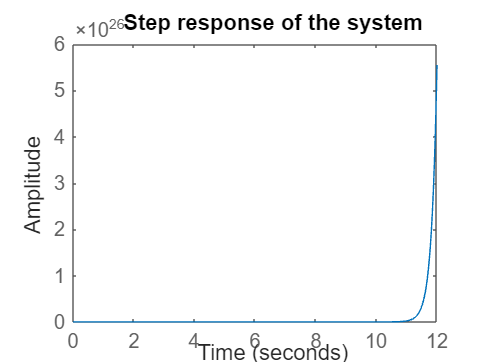
\includegraphics[width=0.7\textwidth]{step.png} % Adjust path to your image
    \caption{Step Response of the System}
\end{figure}

\subsection*{2.3 Controllability and Observability}
The ranks of the controllability and observability matrices are both full (\( \text{Rank} = 4\)), confirming that the system is controllable and observable.
\begin{figure}[h!]
    \centering
    \begin{minipage}{0.45\textwidth}
        \centering
        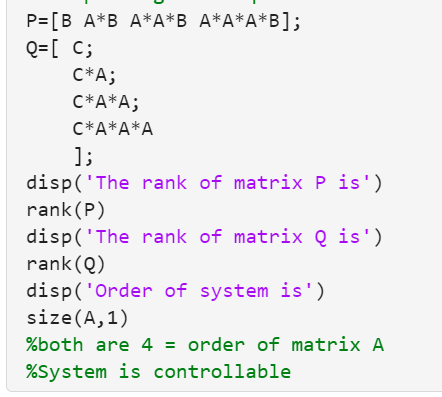
\includegraphics[width=\textwidth]{rank.png}
        \caption{Code for Controllability and Observability}
    
    \end{minipage}
    \hfill
    \begin{minipage}{0.45\textwidth}
        \centering
        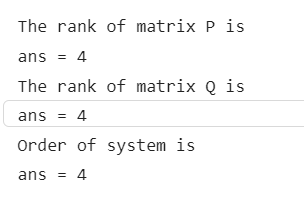
\includegraphics[width=\textwidth]{rank_output.png}
        \caption{Output of Controllability and Observability}
        
    \end{minipage}
\end{figure}
\subsection*{2.4 Controller and Observer Design}
- \textbf{State-Feedback Controller (SFC):} The controller gain matrix is:
\[
K = \begin{bmatrix} -10.7754 & -7.8698 & 37.9423 & 7.3679 \end{bmatrix}
\]
- \textbf{Observer Feedback Controller (OFC):} The observer gain matrix is:
\[
L = \begin{bmatrix}
0.0212 \\ 0.1849 \\ 0.4650 \\ 2.5916
\end{bmatrix}
\]
- Closed-loop system matrices:
\[
A_{clp} = A - BK, \quad A_{clp2} = A - LC
\]

\begin{figure}[h!]
    \centering
    \begin{minipage}{0.45\textwidth}
        \centering
        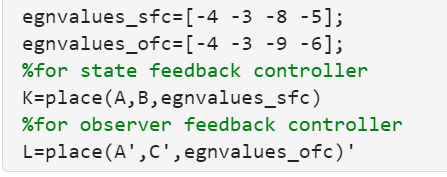
\includegraphics[width=\textwidth]{eigen_values.png}
        \caption{Code for K and L matrices}
    
    \end{minipage}
    \hfill
    \begin{minipage}{0.45\textwidth}
        \centering
        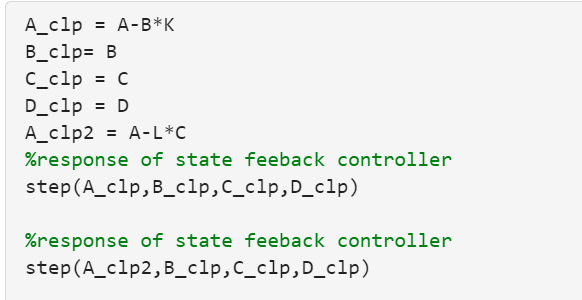
\includegraphics[width=\textwidth]{responses_code.png}
        \caption{Code for state feedback and observer feedback controller}
    \end{minipage}
\end{figure}

\begin{figure}[h!]
    \centering
    \begin{minipage}{0.45\textwidth}
        \centering
        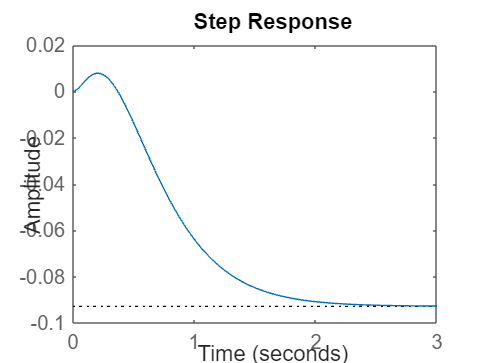
\includegraphics[width=\textwidth]{state_feedback.png}
        \caption{Response for State Feedback Controller}
    
    \end{minipage}
    \hfill
    \begin{minipage}{0.45\textwidth}
        \centering
        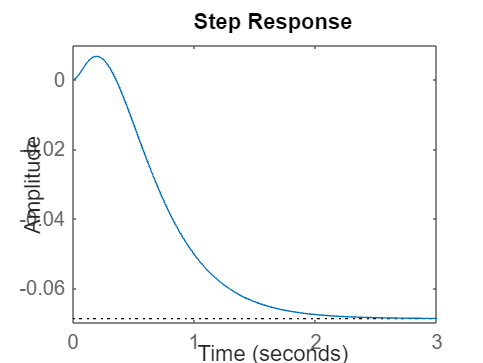
\includegraphics[width=\textwidth]{observer_feedback.png}
        \caption{Response for Observer Feedback Controller}
    \end{minipage}
\end{figure}

\subsection*{2.5 PID Controller Design}
The PID controller parameters are:
\[
K_p = -0.0552, \quad K_i = -0.000684, \quad K_d = -1.11
\]

The closed-loop system transfer function is:
\[
\text{sys}_{\text{now}} =
\frac{-2.024s^4 - 0.1003s^3 + 49.6s^2 + 2.458s + 0.03046}
{s^5 - 1.206s^4 - 31.28s^3 + 25.3s^2 + 2.458s + 0.03046}
\]
\newpage
The step response of the system with PID controller is:
\begin{figure}[H]
    \centering
    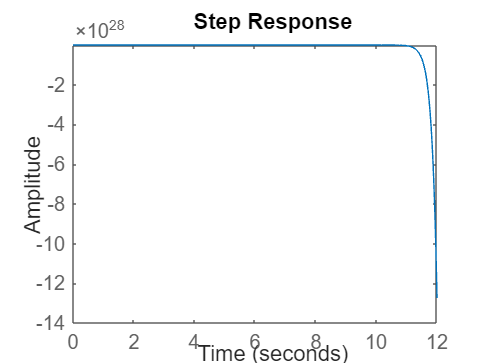
\includegraphics[width=0.7\textwidth]{PID.png}
    \caption{Response for PID Controller}
\end{figure}


\subsection*{2.6 Simulation Results}
Step response of the system confirms performance improvement with controllers.DC gains before and after controllers:
\[
\text{DC gain (Open-loop)} = \infty, \quad
\text{DC gain (SFC)} = -0.0928, \quad
\text{DC gain (OFC)} = -0.0687, \quad
\text{DC gain (PID)} = 1
\]

- Steady-state errors:
\[
\text{Error (Open-loop)} = 0, \quad
\text{Error (SFC)} = 1.1023, \quad
\text{Error (OFC)} = 1.0738, \quad
\text{Error (PID)} = 0.5
\]
\begin{figure}[h!]
    \centering
    \begin{minipage}{0.5\textwidth}
        \centering
        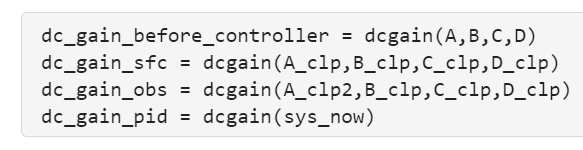
\includegraphics[width=\textwidth]{dcgain.png}
        \caption{DC gain code}
       
    \end{minipage}
    \hfill
    \begin{minipage}{0.45\textwidth}
        \centering
        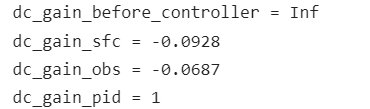
\includegraphics[width=\textwidth]{dcgain_output.png}
        \caption{DC gain Output}
    
    \end{minipage}

\end{figure}
\begin{figure}[H]
    \centering
    \begin{minipage}{0.45\textwidth}
        \centering
        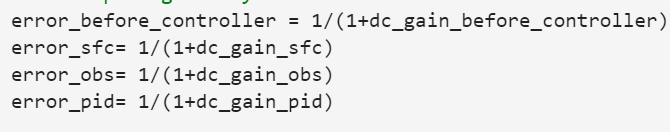
\includegraphics[width=\textwidth]{error.png}
        \caption{Error code}
     
    \end{minipage}
    \hfill
    \begin{minipage}{0.45\textwidth}
        \centering
        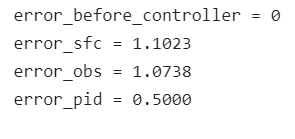
\includegraphics[width=\textwidth]{error_output.png}
        \caption{Error Output}
    \end{minipage}
\end{figure}

\section*{3. Results and Discussion}
This section summarizes the results obtained from the simulations and discusses the implications of the findings. The project successfully demonstrates the design and analysis of controllers for an unstable system. The MATLAB simulations validate the improvements in system dynamics and performance, confirming the effectiveness of the designed controllers.

\begin{figure}[h!]
    \centering
    \begin{minipage}{1\textwidth}
        \centering
        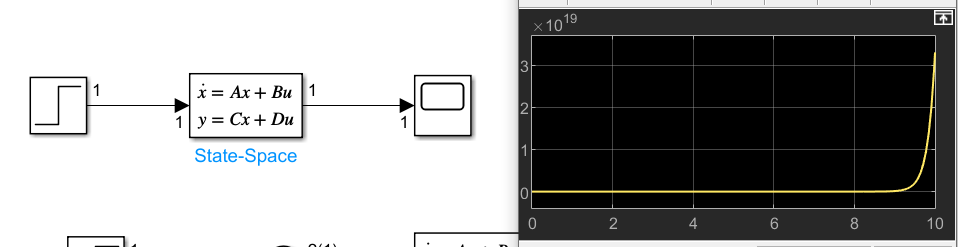
\includegraphics[width=\textwidth]{simulink_system_response.png}
        \caption{Simulink System Response}
    
    \end{minipage}
    \begin{minipage}{1\textwidth}
        \centering
        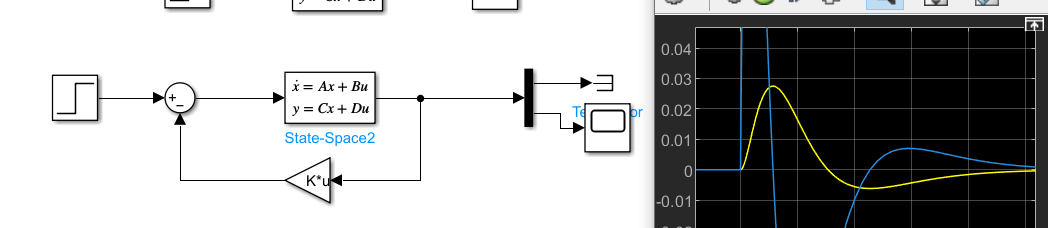
\includegraphics[width=\textwidth]{sl_sfc.png}
        \caption{Simulink State Feedback Controller}
    \end{minipage}
    \begin{minipage}{1\textwidth}
        \centering
        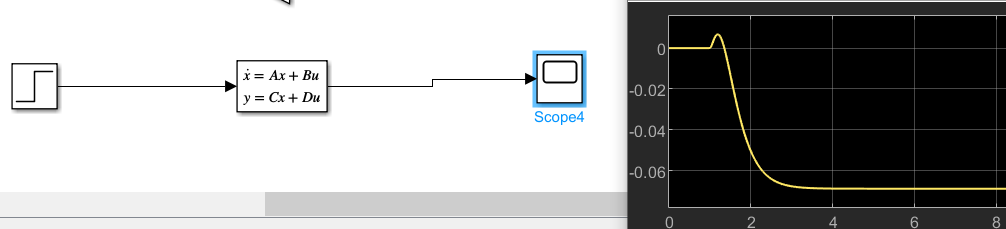
\includegraphics[width=\textwidth]{sl_obs.png}
        \caption{Simulink Observer Feedback Controller}
    \end{minipage}
    \begin{minipage}{1\textwidth}
        \centering
        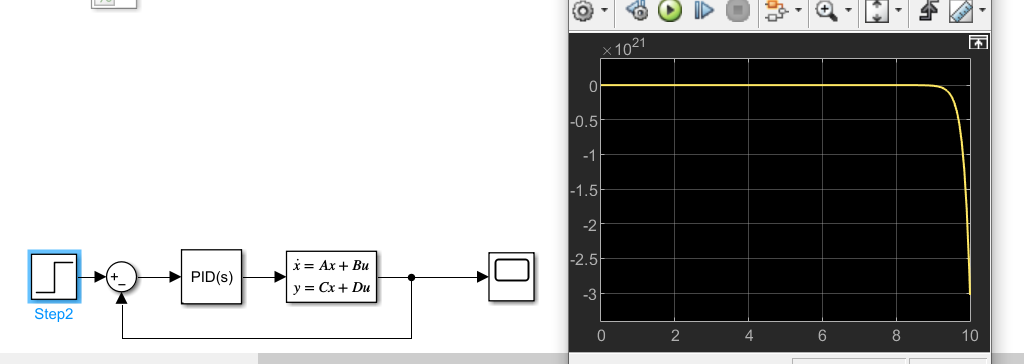
\includegraphics[width=\textwidth]{sl_PID.png}
        \caption{Simulink PID Feedback Controller}
    \end{minipage}
\end{figure}
\end{document}
